	\chapter{\phantom{title}}

\lettrine{A}{}\emph{spiritu fornicatiouis,}

\emph{Domine, libera nos.}

Dal lampo e dalla tempesta,

Liberaci, Signore.

Dal flagello del terremoto,

Liberaci, Signore.

Dalla peste, dalla carestia e dalla guerra,

Liberaci, Signore.

Dal luogo del suolo zero,

Liberaci, Signore.

Dalla pioggia del cobalto,

Liberaci, Signore.

Dalla pioggia dello stronzio,

Liberaci, Signore.

Dalla caduta del cesio,

Liberaci, Signore.

Dalla maledizione del Fallout,

Liberaci, Signore.

Dal generare i mostri,

Liberaci, Signore.

Dalla maledizione del Malnato,

Liberaci, Signore.

\emph{A morte perpetua,}

\emph{Domine, libera nos.}

\emph{Peccatores,}

\emph{Te rogamus, audi nos.}

Che Tu ci risparmi,

noi Ti supplichiamo, ascoltaci.

Che Tu ci perdoni,

noi Ti supplichiamo, ascoltaci.

Che Tu ci conduca alla vera penitenza,

noi Ti supplichiamo, ascoltaci.

~
Frammenti di simili versetti dalle Litanie dei santi uscivano
sussurrando a ogni respiro ansimante di frate Francis mentre si calava
imbarazzato lungo la scala dell\textquotesingle antico Rifugio
Sopravvivenza Fallout, armato com\textquotesingle era soltanto della sua
acqua santa e di una torcia improvvisata, accesa sulle braci serbate dal
fuoco della notte precedente. Aveva atteso per più di
un\textquotesingle ora che qualcuno venisse dall\textquotesingle abbazia
per indagare sul vortice di polvere. E nessuno era venuto.

Abbandonare anche per breve tempo la vigilia vocazionale, a meno di
essere gravemente ammalato o di aver ricevuto l\textquotesingle ordine
di ritornare all\textquotesingle abbazia sarebbe stato considerato come
una rinuncia \emph{ipso facto} alla sua pretesa d\textquotesingle una
vocazione sincera alla vita monastica nell\textquotesingle Ordine
Albertiano di Leibowitz. Frate Francis avrebbe preferito la morte.
Perciò si era trovato di fronte a un dilemma: o ispezionare la
spaventevole fossa prima del tramonto, o trascorrere la notte nella sua
tana senza sapere cosa si potesse nascondere nel rifugio, qualcosa che
avrebbe potuto destarsi e venire a cercarlo
nell\textquotesingle oscurità. Come rischio notturno, i lupi erano già
abbastanza terribili, e i lupi erano soltanto creature di carne e di
sangue. Creature di sostanza meno solida, Francis preferiva incontrarle
alla luce del giorno; sebbene, per la verità, la luce del giorno adesso
cadesse obliquamente nella fossa sottostante, poiché il sole era già
basso, a occidente.

I detriti che erano crollati nel rifugio formavano una collinetta che
aveva la cresta vicino alla sommità delle scale, e lì
c\textquotesingle era soltanto uno strettissimo passaggio fra le pietre
e il soffitto. Vi entrò a piedi in avanti e si trovò costretto a
continuare nello stesso modo, a causa della pendenza molto ripida. Poi,
affrontando l\textquotesingle Ignoto faccia-a-schiena, cercò un sostegno
per i piedi sui mucchi malfermi di pietre spezzate e si fece
gradualmente strada verso il basso.

Di tanto in tanto, quando la sua torcia sembrava che stesse per
spegnersi, si fermava un momento per inclinare la fiamma verso il basso,
lasciando che il fuoco risalisse lungo il legno; durante quelle pause,
cercava di valutare il pericolo che lo circondava e quello che lo
attendeva più sotto. C\textquotesingle era ben poco da vedere. Era in
una stanza sotterranea, ma almeno un terzo di questa era riempito dal
mucchio di detriti che era caduto dalla tromba delle scale.

La cascata di pietre aveva coperto tutto il pavimento, fracassato
parecchi mobili che egli poteva vedere; e probabilmente ne aveva sepolti
altri completamente. Vide alcuni armadietti metallici tutti ammaccati e
con le ante piegate, sepolti per metà nelle macerie.
All\textquotesingle estremità della stanza poteva vedere una porta
metallica, montata su cardini che le avrebbero permesso di aprirsi verso
l\textquotesingle esterno, e sigillata dalla valanga. Ancora leggibili,
a dispetto della vernice scrostata, c\textquotesingle erano sulla porta
queste parole:

\begin{center}
	{\Large PORTELLO INTERNO}
\end{center}

\begin{center}
	{\Large AMBIENTE SIGILLATO}
\end{center}

Evidentemente la stanza in cui era disceso era soltanto
un\textquotesingle anticamera. Ma qualsiasi cosa vi fosse al di là del
PORTELLO INTERNO era sigillata da parecchie tonnellate di roccia che
premevano contro la porta. Il suo ambiente era veramente SIGILLATO a
meno che non vi fosse un\textquotesingle altra uscita.

Dopo essere giunto ai piedi del pendio, e dopo essersi assicurato che
l\textquotesingle anticamera non contenesse alcuna minaccia manifesta,
il novizio andò a ispezionare cautamente la porta metallica più da
vicino, al lume della torcia. Sotto la scritta PORTELLO INTERNO
c\textquotesingle era una targa più piccola, striata di ruggine:

\begin{center}
	\justify{AVVERTENZA: Questo portello non deve essere chiuso prima che tutto il
		personale sia entrato, o prima che siano state predisposte tutte le
		misure di sicurezza prescritte dal Manuale Tecnico CD-Bu-83A. Quando il
		portello è chiuso, l\textquotesingle aria nell\textquotesingle interno
		del rifugio sarà pressurizzata a 2,0 psi al di sopra del livello
		barometrico ambiente per minimizzare la diffusione interna. Una volta
		sigillato, il portello sarà aperto automaticamente dal sistema
		servo-monitor allorché (ma non prima) prevarrà una delle seguenti
		condizioni: 1) quando la radiazione esterna scenderà al di sotto del
		livello pericoloso; 2) qualora i sistemi di ripurificazione
		dell\textquotesingle acqua e dell\textquotesingle aria si guastassero;
		3) qualora la riserva di cibo si esaurisse; 4) qualora si guastasse
		l\textquotesingle impianto elettrico interno. Vedere CD-Bu-83A per
		ulteriori istruzioni.}
\end{center}
\leavevmode\\
Frate Francis si sentì lievemente confuso da
quell\textquotesingle Avvertenza ma pensò di rispettarla non toccando
affatto la porta. I miracolosi aggeggi degli antichi non dovevano essere
manomessi spensieratamente, come molte volte i dissotterratori del
passato avevano testimoniato con il loro ultimo respiro.

Frate Francis osservò che i detriti rimasti per secoli
nell\textquotesingle anticamera erano di colore più scuro e di grana più
ruvida dei detriti che erano stati sottoposti
all\textquotesingle inclemenza del sole e della sabbia prima del crollo
di quel giorno.

Si poteva capire, con un\textquotesingle occhiata alle pietre, che il
Portello Interno era stato bloccato non dalla frana di quel giorno ma da
un\textquotesingle altra, molto più antica della stessa abbazia. Se
l\textquotesingle Ambiente Sigillato del Rifugio Sopravvivenza Fallout
conteneva un Fallout, il demone non aveva evidentemente aperto il
Portello Interno dal tempo del Diluvio di Fiamma, prima della
Semplificazione. E, se era rimasto sigillato dietro la porta di metallo
per tanti secoli, c\textquotesingle era ben poca ragione, si disse
Francis, di temere che potesse irrompere dal portello prima del Sabato
Santo.

La fiamma della torcia si abbassò. Trovò una gamba fracassata
d\textquotesingle una sedia, l\textquotesingle accese con la sua fiamma
vacillante, poi cominciò a raccogliere pezzi di mobilio rotto per
accendere un vero fuoco, mentre ponderava il significato
dell\textquotesingle antica targa: RIFUGIO SOPRAVVIVENZA FALLOUT.

Come frate Francis ammise prontamente, la sua padronanza
dell\textquotesingle inglese prediluviale era ben lontana
dall\textquotesingle essere perfetta. Il modo in cui i sostantivi
potevano talvolta modificare altri sostantivi, in quella lingua, era
sempre stato uno dei suoi punti deboli. Nel latino, come nei più
semplici dialetti della regione, una costruzione, come \emph{servus
	puer} significava la stessa cosa che \emph{puer servus}, e anche in
inglese \emph{slave boy} significava \emph{boy slave}, ragazzo schiavo.
Ma qui le somiglianze finivano. Alla fine era riuscito a imparare che
\emph{house cat} non significava \emph{cat house} e che un dativo di
scopo o possessivo, come in \emph{mihi amicus}, equivaleva pressappoco a
\emph{dog food} o a \emph{sentry boy}, anche senza inflessione. Ma cosa
significava una tripla apposizione come rifugio sopravvivenza fallout,
\emph{fallout survival shelter}? Frate Francis scosse il capo.
L\textquotesingle avvertenza sul portello interno parlava di cibo, di
acqua e di aria; e senza dubbio non erano cose necessarie per i maligni
dell\textquotesingle Inferno. Qualche volta, il novizio trovava
l\textquotesingle inglese prediluviale più difficile
dell\textquotesingle Angelologia Intermedia o del Calcolo Teologico di
san Leslie.

Accese il fuoco sul pendio del mucchio di macerie, dove avrebbe potuto
illuminare gli angoli più bui dell\textquotesingle anticamera. Poi andò
a esplorare tutto ciò che poteva essere rimasto scoperto dai detriti. Le
rovine a fior di terra erano state ridotte ad ambiguità archeologiche da
intere generazioni di scavatori, ma questa rovina sotterranea non era
stata toccata se non dalla mano di un disastro impersonale. Il luogo
sembrava infestato da presenze di un\textquotesingle altra età. Un
cranio, che giaceva fra le pietre in un angolo più buio, aveva ancora un
dente d\textquotesingle oro nel suo ghigno\ldots{} chiara dimostrazione
che il rifugio non era stato invaso dai vagabondi.
L\textquotesingle incisivo d\textquotesingle oro scintillava, quando il
fuoco danzava più alto.

Più di una volta frate Francis aveva incontrato, nel deserto, vicino a
qualche torrente prosciugato, un mucchietto di ossa umane, ripulite e
imbiancate dal sole. Non era particolarmente schizzinoso ed era
preparato a simili scene. Perciò Francis non fu sorpreso quando notò il
cranio nell\textquotesingle angolo dell\textquotesingle anticamera, ma
lo scintillio d\textquotesingle oro in quel ghigno attirava
continuamente il suo sguardo mentre tentava di aprire gli sportelli
(chiusi a chiave o incastrati) degli armadietti rugginosi, o i cassetti
(egualmente incastrati) di una scrivania metallica tutta ammaccata. La
scrivania poteva rivelarsi una scoperta inestimabile, se conteneva
documenti o un paio di libri sfuggiti ai furibondi roghi
dell\textquotesingle Età della Semplificazione. Mentre insisteva nei
tentativi di aprire i cassetti, la fiamma si abbassò; ebbe
l\textquotesingle impressione che il teschio cominciasse a emettere un
debole bagliore proprio. Un fenomeno del genere non era particolarmente
insolito, ma nella cripta buia, frate Francis lo giudicò molto
conturbante. Raccolse altra legna per il fuoco, ritornò a scuotere i
cassetti della scrivania, cercando di ignorare il ghigno scintillante
del teschio. Sebbene avesse ancora timore dei Fallout nascosti, Francis
si era ripreso dallo spavento iniziale quel tanto che bastava per
comprendere che il rifugio, specialmente la scrivania e gli armadietti,
potevano essere pieni di ricche reliquie d\textquotesingle una età che
il mondo, per la maggior parte, aveva preferito dimenticare.

La Provvidenza aveva elargito una vera benedizione, qui. Trovare un
frammento del passato sfuggito ai roghi e ai predatori era un raro colpo
di fortuna, in quei tempi. Tuttavia, questo sottintendeva un rischio. Si
sapeva che gli scavatori monastici, attenti ai tesori antichi,
emergevano talvolta da una buca nel terreno, recando trionfalmente un
bizzarro oggetto cilindrico e poi --- mentre lo ripulivano o cercavano
di scoprirne la funzione --- premevano il pulsante sbagliato o giravano
l\textquotesingle interruttore sbagliato, e così ponevano fine alla
intera faccenda senza alcun beneficio per il clero. Soltanto ottanta
anni prima il venerabile Boedullus aveva scritto con evidente gioia al
suo Signor Abate che la sua piccola spedizione aveva scoperto i resti,
secondo le sue stesse parole ``del luogo d\textquotesingle una pista di
lancio intercontinentale, completa di parecchi, affascinanti serbatoi
sotterranei''. Nessuno, nell\textquotesingle abbazia, aveva mai saputo
cosa intendesse il venerabile Boedullus per ``pista di lancio
intercontinentale'', ma il Signor Abate che regnava a quel tempo aveva
severamente decretato che gli antiquari monastici dovevano, sotto pena
di scomunica, evitare quelle ``piste'', per l\textquotesingle avvenire.
Perché la sua lettera all\textquotesingle abate era stata
l\textquotesingle ultima cosa che si era vista del venerabile Boedullus,
della sua spedizione, della sua ``pista di lancio'' e del piccolo
villaggio che sorgeva in quel luogo: adesso un lago molto interessante
aggraziava il paesaggio, dove era stato il villaggio, grazie ad alcuni
pastori che avevano deviato il corso di un ruscello e
l\textquotesingle avevano fatto scorrere nel cratere, per raccogliervi
acqua per le loro greggi nei tempi di siccità. Un viaggiatore che era
venuto da quella direzione circa un decennio prima aveva riferito che in
quel lago si facevano pesche eccellenti, ma i pescatori dei dintorni
consideravano i pesci come se fossero le anime degli scavatori e degli
abitanti del villaggio rimasti uccisi molto tempo prima: e rifiutavano
di pescare a causa di Bo\textquotesingle dollos, il pesce gatto
gigantesco che vi viveva nel profondo.

``\ldots{} né alcuno scavo verrà iniziato se non avrà come principale
scopo l\textquotesingle accrescimento dei Memorabilia'' aveva aggiunto
il decreto del Signor Abate\ldots{} Questo significava che frate Francis
doveva frugare il rifugio soltanto per cercare libri e documenti, senza
maneggiare eventuali strumenti e utensili.

Il dente d\textquotesingle oro continuava ad ammiccare e a scintillare
in un angolo dei suoi occhi mentre frate Francis cercava di aprire i
cassetti della scrivania. I cassetti rifiutavano di muoversi. Diede un
calcio finale alla scrivania e si voltò a guardare impaziente il
teschio: ``Perché non sogghigni verso qualcosa d\textquotesingle altro,
tanto per cambiare?''.

Il sogghigno rimase. La reliquia dal dente d\textquotesingle oro giaceva
con il capo appoggiato fra una pietra e una cassetta di metallo
arrugginito. Lasciando la scrivania, il novizio si fece strada fra i
detriti per esaminare finalmente da vicino quei resti mortali. Era
chiaro che quella persona era morta in quel punto, investita dal
torrente di pietre e semisepolta dalle macerie. Solo il teschio e le
ossa d\textquotesingle una gamba non erano stati ricoperti. Il femore
era spezzato, la parte posteriore del cranio era sfracellata.

Frate Francis sussurrò una preghiera per il defunto, poi, con grande
delicatezza, sollevò il teschio dal punto in cui riposava e lo girò in
modo che sogghignasse verso la parete. Quindi il suo sguardo cadde sulla
cassetta arrugginita.

La cassetta aveva la forma d\textquotesingle una cartella da scolaro ed
era evidentemente una specie di valigia. Poteva essere servita a molti
usi, ma era stata malamente ammaccata dalle pietre nella loro caduta. La
liberò goffamente dalle macerie e la portò più vicino al fuoco. La
serratura sembrava rotta, ma il coperchio era stato quasi saldato dalla
ruggine. La cassetta emise un rumore metallico, quando la scosse. Non
era la custodia più adatta per cercarvi libri o documenti, ma era
evidente che era stata costruita per essere aperta e chiusa, e poteva
contenere qualche frammento di informazione per i Memorabilia. Tuttavia,
ricordando il destino di frate Boedullus e di altri,
l\textquotesingle asperse di acqua santa prima di tentare di aprirla, e
maneggiò l\textquotesingle antica reliquia con la massima reverenza
possibile mentre batteva con una pietra sui cardini arrugginiti,

Finalmente ruppe i cardini, e il coperchio si staccò. Minuscoli
frammenti metallici, schizzarono dagli scomparti, si sparsero fra le
rocce; qualcuno si perdette nei crepacci. Ma, sul fondo della cassetta,
nello spazio sotto agli scomparti scorse\ldots{} dei documenti! Dopo una
breve preghiera di ringraziamento, raccolse tutti i frammenti metallici
che poté e, dopo aver riabbassato il coperchio, cominciò a salire la
collinetta di detriti verso la tromba delle scale e verso la piccola
striscia di cielo, tenendo ben stretta la cassetta sotto un braccio.

Il sole era accecante, dopo l\textquotesingle oscurità del rifugio. Non
si accorse nemmeno che stava scendendo pericolosamente verso
l\textquotesingle orizzonte, a occidente, ma cominciò immediata-niente a
cercare una lastra piatta sulla quale poter spargere il contenuto della
cassetta per esaminarlo senza correre il rischio di perdere qualcosa
nella sabbia.

Qualche minuto più tardi, seduto su una pietra screpolata alle
fondamenta, cominciò a togliere i pezzetti di metallo e di vetro che
riempivano gli scomparti. Molti erano piccoli oggetti tubolari con un
filamento metallico a ogni estremità. Ne aveva già visti, prima
d\textquotesingle allora. Il piccolo museo dell\textquotesingle abate ne
possedeva qualcuno, di varia grandezza, forma e colore. Una volta aveva
visto uno sciamano del popolo pagano delle colline che ne indossava una
fila come collana cerimoniale. Il popolo delle colline li considerava
come ``parti del corpo del dio''\ldots{} della favolosa \emph{Machina
	analytica}, osannata come il più saggio dei loro dei. Ingoiando uno di
quegli oggetti, uno sciamano poteva acquisire
l\textquotesingle Infallibilità, dicevano. Senza dubbio, in quel modo
acquisiva l\textquotesingle Indiscutibilità, fra la sua gente\ldots{} a
meno che ne inghiottisse uno del tipo velenoso. Gli oggettini del museo
erano egualmente collegati gli uni agli altri\ldots{} non sotto forma di
collana, ma come un labirinto complesso e piuttosto disordinato in fondo
a una piccola cassetta di metallo, etichettata come: ``Chassis Radio:
Applicazione Incerta''.

Nell\textquotesingle interno del coperchio della cassetta, era stato
incollato un foglietto; la colla si era polverizzata,
l\textquotesingle inchiostro era sbiadito e la carta era così macchiata
di ruggine che persino una buona grafia sarebbe stata difficile da
leggere, e questa era una scritta scarabocchiata in fretta. La studiò, a
intermittenze, mentre vuotava gli scomparti. Sembrava una specie di
inglese, ma passò mezz\textquotesingle ora prima che riuscisse a
decifrare quasi tutto il messaggio:

\begin{center}
	CARL\ldots{}
\end{center}

\begin{center}
	\justify{devo prendere l\textquotesingle aereo per (indecifrabile) fra venti
			minuti. Per amor di Dio, tieni lì Em fino a che sapremo se siamo o no in
			guerra. Ti prego, cerca di farla mettere nell\textquotesingle elenco di
			riserva per il rifugio. Non sono riuscito a procurarle un posto sul mio
			aereo. Non dirle perché te l\textquotesingle ho mandata con questa
			cassetta di cianfrusaglie, ma cerca di tenerla li finché non sapremo
			(indecifrabile) nella peggiore delle ipotesi, uno dei convocati di
			riserva non si faccia vivo.}
\end{center}

\begin{center}
	I.E.L.
\end{center}

\begin{center}
	\justify{P.S. --- Metto il sigillo sulla serratura e scrivo SEGRETISSIMO sul
			coperchio per impedire a Em di guardarci dentro. È la prima cassetta che
			mi sono trovato a portata di mano. Scaraventala nel mio armadietto o
			qualcosa del genere.}
\end{center}

Quel biglietto sembrò un fugace balbettio infantile a frate Francis, che
in quel momento era troppo eccitato per concentrarsi su un solo
particolare. Dopo una ironica occhiata finale ai frettolosi scarabocchi,
si accinse al compito di togliere gli scomparti per arrivare alle carte
che si trovavano in fondo alla cassetta. Gli scomparti erano tutti
montati su supporti che evidentemente dovevano servire a staccare gli
scomparti stessi dalla cassetta, se la si teneva fortemente inclinata,
ma i sostegni erano arrugginiti e frate Francis fu costretto a smuoverli
servendosi di un piccolo strumento d\textquotesingle acciaio prelevato
da uno degli scomparti.

Quando frate Francis ebbe tolto l\textquotesingle ultimo scomparto,
toccò con reverenza le carte; c\textquotesingle era solo una manciata di
documenti ripiegati, eppure era un vero tesoro; perché quelle carte
erano sfuggite alle fiamme colleriche della Semplificazione, in cui si
erano arricciati, anneriti e avvizziti trasformandosi in fumo persino
scritti sacri, mentre la folla ignorante ululava e gridava in trionfo.

Maneggiò con massima cura le carte come avrebbe potuto maneggiare
oggetti sacri, riparandole dal vento con il suo abito poiché erano tutte
fragili, screpolate dal tempo. C\textquotesingle era un fascio di rozzi
disegni e diagrammi. C\textquotesingle erano biglietti, scritti a mano,
due grandi fogli piegati e un libriccino in- titolato \emph{Memorandum}.

Per prima cosa esaminò i biglietti. Erano scarabocchiati dalla stessa
mano che aveva scritto la nota incollata al coperchio della cassetta
metallica, e la grafia non era meno abominevole. \emph{Un etto
	pasticcini}, diceva un biglietto, \emph{scatola crauti\ldots{} portare a
	casa per Emma}. Un altro rammentava: \emph{Ricordare\ldots{} cercare il
	modulo 1040, Zio Fisco}. Un altro biglietto era solamente una colonna di
numeri il cui totale era delimitato da un segno circolare; da questo
totale veniva sottratta una seconda somma e finalmente veniva tratta una
percentuale, seguita dalla parola \emph{accidenti!}

Frate Francis controllò i conti: non riuscì a trovare errori
nell\textquotesingle aritmetica di quell\textquotesingle abominevole
calligrafo, per lo meno, anche se non poté dedurre che cosa
rappresentassero tutte quelle quantità.

Maneggiò il \emph{Memorandum} con speciale reverenza, perché il suo
titolo faceva pensare al Memorabilia. Prima di aprirlo, si fece il segno
della croce e mormorò la Benedizione dei Testi. Ma il libriccino fu una
delusione. Si era aspettato un\textquotesingle opera stampata, ma trovò
soltanto un elenco manoscritto di nomi, luoghi, numeri e date. Le date
andavano dall\textquotesingle ultima parte del quinto decennio alla
prima parte del sesto, secolo XX. Una nuova conferma! Il contenuto del
rifugio proveniva dal periodo crepuscolare dell\textquotesingle Età
dell\textquotesingle Illuminazione. Era veramente una scoperta
importante.

Dei fogli più grandi, uno era strettamente arrotolato; e cominciò a
rompersi quando frate Francis cercò di srotolarlo; riuscì a capire le
parole PROGRAMMA DELLE CORSE, ma nient\textquotesingle altro. Dopo
averlo nuovamente riposto nella cassetta per un successivo lavoro di
restauro, si occupò del secondo documento ripiegato: era così
estremamente fragile che osò esaminarne soltanto una parte, aprendo
leggermente le falde e sbirciandovi in mezzo.

Un diagramma, sembrava, ma.. un diagramma di linee bianche su carta
scura!

Ancora una volta provò l\textquotesingle eccitazione della scoperta. Era
evidentemente una \emph{blueprint\ldots{}} e
nell\textquotesingle abbazia non c\textquotesingle era una sola
\emph{blueprint} originale, ma solo facsimili a inchiostro. Gli
originali erano sbiaditi da molto tempo, a causa
dell\textquotesingle eccessiva esposizione alla luce. Mai, prima di
allora, frate Francis aveva visto un originale, anche se aveva visto
abbastanza riproduzioni dipinte a mano per poter riconoscere una
\emph{blueprint} che, sebbene macchiata e scolorita, era ancora
leggibile dopo tanti secoli, a causa della totale oscurità e della
scarsa umidità del rifugio in cui era rimasta.

Rovesciò il documento.., e provò un breve impulso di furore. Chi era
stato l\textquotesingle idiota che aveva sfregiato quel documento
inestimabile? Qualcuno aveva distrattamente scarabocchiato figure
geometriche e puerili facce caricaturali sul verso del foglio. Chi era
stato quel vandalo sconsiderato\ldots{}

L\textquotesingle ira svanì dopo un istante di riflessione. Al tempo del
misfatto, probabilmente le \emph{blueprints} erano state comuni quanto
l\textquotesingle erba, e il proprietario della cassetta era il
probabile colpevole. Riparò il foglio dal sole con la propria ombra,
mentre cercava di aprirlo. Nell\textquotesingle angolo. inferiore destro
c\textquotesingle era un rettangolo stampato che conteneva, in lettere
semplici, vari titoli, date, ``numeri dei brevetti'', numeri di
riferimento e nomi. Il suo sguardo scese lungo l\textquotesingle elenco
fino a che incontrò: DISEGNO DEL CIRCUITO: \emph{Leibowitz, I.E.}

Chiuse per un momento gli occhi e scosse il capo fino a che gli parve di
sentirlo tintinnare. Poi guardò di nuovo.. Era li, molto chiaro:

\begin{center}
	DISEGNO DEL CIRCUITO: \emph{Leibowitz, I.E.}
\end{center}

Rovesciò di nuovo il foglio. Fra le figure geometriche e gli schizzi
puerili, chiaramente stampigliato in inchiostro purpureo,
c\textquotesingle era il timbro:

\begin{figure}[h]
	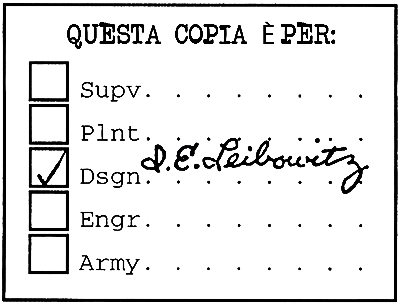
\includegraphics[scale=0.4]{Immagini/timbro.png}
	\centering
\end{figure}

~

Il nome era scritto in una nitida grafia femminile, non con i frettolosi
scarabocchi degli altri appunti. Guardò di nuovo le iniziali che
siglavano il biglietto incollato al coperchio della cassetta:
I.E.L\ldots{} e poi DISEGNO DEL CIRCUITO\ldots{} E le stesse iniziali
apparivano in altri punti, nelle annotazioni.

C\textquotesingle erano state discussioni, puramente congetturali per
decidere se il beato fondatore dell\textquotesingle Ordine, se fosse
stato finalmente canonizzato, avrebbe dovuto essere invocato come san
Isaac o san Edward. Qualcuno aveva proposto san Leibowitz, poiché, fino
a quel momento, era stato chiamato per cognome.

--- \emph{Beate Leibowitz, ora pro me!} --- sussurrò Francis. Le mani
gli tremavano così forte che minacciavano di rovinare i fragili
documenti. Aveva scoperto delle reliquie del Santo. Naturalmente, Nuova
Roma non aveva ancora proclamato Leibowitz santo, ma frate Francis ne
era così convinto che osò aggiungere: --- \emph{Sancte Leibowitz, ora
	pro me!}

Frate Francis non sprecò alcuna logica oziosa nel balzare immediatamente
alla conclusione: gli era stato concesso dal Cielo un segno della sua
vocazione. Aveva trovato ciò che aveva dovuto cercare nel deserto, come
la vedeva lui. Era chiamato a diventare monaco professo
dell\textquotesingle Ordine. Dimenticando che l\textquotesingle abate
ammoniva severamente di non attendersi che una vocazione venisse in
forma spettacolare o miracolosa, il novizio si inginocchiò sulla sabbia
per una preghiera di ringraziamento e per offrire qualche decina del
rosario per il vecchio pellegrino che gli aveva indicato la pietra che
conduceva al rifugio. \emph{Ti auguro di trovare presto la Voce,
	figliolo}, aveva detto il viandante. Fino a quel momento il novizio non
aveva sospettato che il pellegrino avesse alluso a una \emph{Voce} con
la V maiuscola.

\emph{``Ut solius tuae voluntatis mihi cupidus sim, et vocationis tuae
	conscius, si digneris me vocare\ldots''}

Sarebbe spettato all\textquotesingle abate decidere se la sua ``voce''
stava parlando il linguaggio delle circostanze e non il linguaggio della
causa e dell\textquotesingle effetto. Sarebbe spettato al \emph{Promotor
	Fidei} pensare che forse Leibowitz non era un cognome insolito prima del
Diluvio di Fiamma che LE. potevano indicare. tanto \emph{Ichabod
	Ebenezer} quanto \emph{Isaac Edward}. Per Francis la possibilità era una
sola.

Dalla lontana abbazia, tre note di campana squillarono attraverso il
deserto, una pausa, poi le tre note furono seguite da altre nove.

--- \emph{Angelus Domini nuntiavit Mariae} --- rispose doverosamente il
novizio, levando sorpreso lo sguardo e accorgendosi che il sole era
divenuto un grosso ovale scarlatto che già toccava
l\textquotesingle orizzonte occidentale. La barriera di pietre attorno
alla sua tana non era ancora completa.

Non appena ebbe recitato l\textquotesingle{}\emph{Angelus}, ripose
frettolosamente le carte nella vecchia cassetta arrugginita. Una
chiamata dal Cielo non comprende necessariamente la facoltà miracolosa
di sottomettere le bestie feroci o di farsi amici i lupi affamati.

Prima che il crepuscolo fosse svanito e che fossero apparse le stelle,
il suo rifugio provvisorio era ben fortificato, per quanto era
possibile; rimaneva solo da verificare che fosse a prova di lupo. Il
collaudo non sarebbe tardato molto. Aveva già udito alcuni ululati
provenire da occidente.

Aveva ravvivato il fuoco, ma non era rimasta alcuna luce, al di là del
cerchio del riverbero delle fiamme, per permettergli di fare la solita
raccolta quotidiana di purpurei frutti di cactus\ldots{} la sua sola
fonte di nutrimento a eccezione delle domeniche, in cui
dall\textquotesingle abbazia venivano mandate poche manciate di grano
secco, dopo che un prete aveva fatto il suo giro con il Santissimo
Sacramento. La lettera della regola per una vigilia quaresimale di
vocazione non era rigorosa quanto la sua applicazione pratica. Così
applicata, la regola equivaleva semplicemente
all\textquotesingle inedia.

Quella notte, tuttavia, i morsi della fame erano per Francis meno
fastidiosi del suo impulso impaziente di correre
all\textquotesingle abbazia ad annunciare la notizia della sua scoperta.
Ma questo avrebbe significato rinunciare alla sua vocazione non appena
discesa su di lui; doveva rimanere lì per la durata della Quaresima,
vocazione o non vocazione, per continuare la sua vigilia come se non
fosse accaduto nulla di straordinario.

Accanto al fuoco, sognando a occhi aperti, guardò
nell\textquotesingle oscurità in direzione del Rifugio Sopravvivenza
Fallout e cercò di immaginare una grande basilica che sorgesse proprio
in quel punto. Era una fantasia piacevole, ma era difficile pensare che
qualcuno scegliesse quella remota zona desertica come centro
d\textquotesingle una futura diocesi. Se non una basilica, almeno una
chiesa più piccola --- la chiesa di San Leibowitz del Deserto ---
circondata da un giardino e da un muro, con una cappella del Santo che
attraeva fiumi di pellegrini dai lombi cinti, provenienti dal Nord.
``Padre'' Francis dello Utah conduceva i pellegrini a fare il giro delle
rovine, li ammetteva persino, al di là del Portello Due, negli splendori
dell\textquotesingle Ambiente Sigillato, le catacombe del diluvio di
Fiamma dove\ldots{} dove\ldots{} bene, dove avrebbe potuto celebrare per
loro la messa sull\textquotesingle altare di pietra che racchiudeva una
reliquia del Santo cui era dedicata quella chiesa\ldots{} un pezzo di
rozzo canovaccio? qualche fibra del cappio del carnefice? ritagli di
unghie trovati in fondo alla cassetta arrugginita?\ldots{} o forse il
PROGRAMMA DELLE CORSE. Ma la fantasia si avvizzì. Le possibilità che
frate Francis diventasse prete erano molto esigue\ldots{} poiché non
appartenevano a un Ordine missionario, i Frati di Leibowitz avevano
bisogno soltanto di un numero di preti sufficienti per
l\textquotesingle abbazia e per poche altre comunità di monaci, in altri
luoghi. Inoltre, il ``Santo'' era ufficialmente ancora un Beato, e non
sarebbe mai stato canonizzato se non avesse compiuto qualche
incontrovertibile miracolo per avvalorare la sua beatificazione, che non
era una proclamazione infallibile come invece sarebbe stata la
canonizzazione, sebbene permettesse formalmente ai monaci
dell\textquotesingle Ordine di Leibowitz di venerare il loro fondatore e
patrono, al di fuori della messa e dell\textquotesingle ufficio. Le
proporzioni della chiesa fantastica si ridussero alle dimensioni
d\textquotesingle una cappelletta, sull\textquotesingle orlo della
strada il fiume di pellegrini si ridusse a un rigagnolo. Nuova Roma era
occupata con altri problemi, come la petizione per dei Doni
Preternaturali della Santa Vergine, poiché i Domenicani sostenevano che
l\textquotesingle Immacolata Concezione comprendeva non soltanto la
grazia innata, ma anche il fatto che la Madre Benedetta avesse avuto i
poteri preternaturali che appartenevano a Eva prima della Caduta; alcuni
teologi di altri Ordini, mentre ammettevano che questa era una
congettura molto pia, negavano che questo fosse il caso in questione, e
sostenevano che una ``creatura'' poteva essere ``monda dal peccato
originale'' ma non dotata di poteri preternaturali. I Domenicani si
inchinavano a questa affermazione, ma sostenevano che la credenza era
sempre stata implicita in altri dogmi: come l\textquotesingle Assunzione
(immortalità preternaturale) e la Preservazione dal Peccato Attuale (che
comprendeva l\textquotesingle integrità preternaturale) e altri esempi
simili. Mentre tentava di risolvere questa disputa, Nuova Roma sembrava
aver lasciato la causa per la canonizzazione di Leibowitz a impolverarsi
sullo scaffale. Accontentandosi d\textquotesingle una piccola cappella
del Beato e di un distratto rigagnolo di pellegrini, frate Francis si
appisolò. Quando si svegliò, il fuoco era ridotto a braci lucenti.
Sembrava che vi fosse qualcosa di sbagliato. Era veramente solo? Si
guardò intorno, battendo le palpebre, nell\textquotesingle oscurità che
lo circondava.

Al di là del letto di carboni rossi, il lupo scuro batté a sua volta le
palpebre.

Il novizio gridò e si tuffò al coperto.

Il grido, decise mentre giaceva tremando nella sua tana di pietre e di
frasche, era stato soltanto una infrazione involontaria alla regola del
silenzio. Giacque, abbracciando la cassetta metallica e pregando che i
giorni della Quaresima passassero in fretta, mentre zampe felpate
raspavano attorno al suo recinto.
